\section{Virtualização}
Como início desta sessão, vamos definir virtualização como uma entidade de software da qual representa um recurso real de hardware, mas não necessariamente representando todas as capacidades deste recurso de hardware, como exemplo, digamos que exista um processador que possua 8 núcleos e 16 threads, mas a virtualização deste recurso representa apenas 4 núcleos e 8 threads deste processador real \cite{virtualizacao_and_cloud}.

\paragraph*{Bases da virtualização}\mbox{}\\
Conforme definições dadas existem alguns critérios para categorização da virtualização, sendo estes as seguintes conforme \cite{Sareen2013CloudCT, virtualizacao_and_cloud}.

\paragraph*{Particionamento}\mbox{}\\
Diversas aplicações e sistemas operacionais (SO) são suportados em um único hardware através da segregação dos recursos, sejam quais estão disponíveis ou uso destes tal como limitação no tráfego de rede.

\paragraph*{Isolamento}\mbox{}\\
Existe o isolamento do uso deste recurso de modo que, mesmo que uma máquina virtual ou container acabe quebrando e finalizando sua execução, não afetará demais aplicações.

\paragraph*{Encapsulamento}\mbox{}\\
Este previne interferência de outros sistemas com demais outros sistemas, devido toda a questão de particionamento dos recursos previamente citado. Desta forma cada ambiente possui recursos e configurações que são próprias para aquele sistema, de modo que temos o software desacoplado do hardware.


\paragraph*{Virtualização e sandbox}\mbox{}\\
Temos a virtualização como base do sandbox, sendo este feito através do isolamento de recursos, sejam estes limitações quanto operações, quanto quantidade de recursos.

Assim sua base gira em torno de um sistema agir de modo intermediário ao hardware e definir quais seriam os recursos que estariam disponíveis para determinado programa ou SO \cite{linux-containers-virtualization}.

Para o uso do conceito sandbox, existem diversas maneiras a serem feitas, e para isto, é necessário compreender algumas categorias de virtualização as quais podem ser utilizadas para seu uso final.

\paragraph*{Categorização da virtualização}\mbox{}\\
A categorização dos tipos de virtualização em alto nível, isto é sem entrar em muitos detalhes conceituais, gira em torno dos tipos de virtualização através de uma máquina virtual (MV) e a conteinerização. Para isso deve-se compreender a diferença entre estes, para que então compare-se e veja como cada um se comporta e porque de ter certas características.

\section{Máquina Virtual (MV)}
\label{chp:referencial_teorico::sct:maquina_virtual}
Temos a MV e esta precisa do hypervisor. Como exemplo digamos que temos um dispositivo de armazenamento o qual interage diretamente com o hypervisor através de seus drivers, o hypervisor gera um driver virtual do qual é utilizado dentro da MV para interagir com o SO convidado \cite{docker_diff_standard_virt}.

O caso da máquina virtual, normalmente é utilizado visando rodar múltiplos SOs diferentes e até de arquiteturas diferentes. Como seu uso implica na utilização de um hypervisor, temos o isolamento dos recursos.

Possuindo em si algumas outras segmentações, tais como a virtualização de tipo 1 (bare-metal) e tipo 2. Como visualização das diferenças entre os tipos de virtualização providos por MVs, temos a figura \ref{fig:virtualization_t1_vs_t2} ilustrativa dos conceitos que serão falados logo a seguir \cite{kernelscheepers, Virtualization_vs_Containerization}.

\begin{figure}
    \centering
    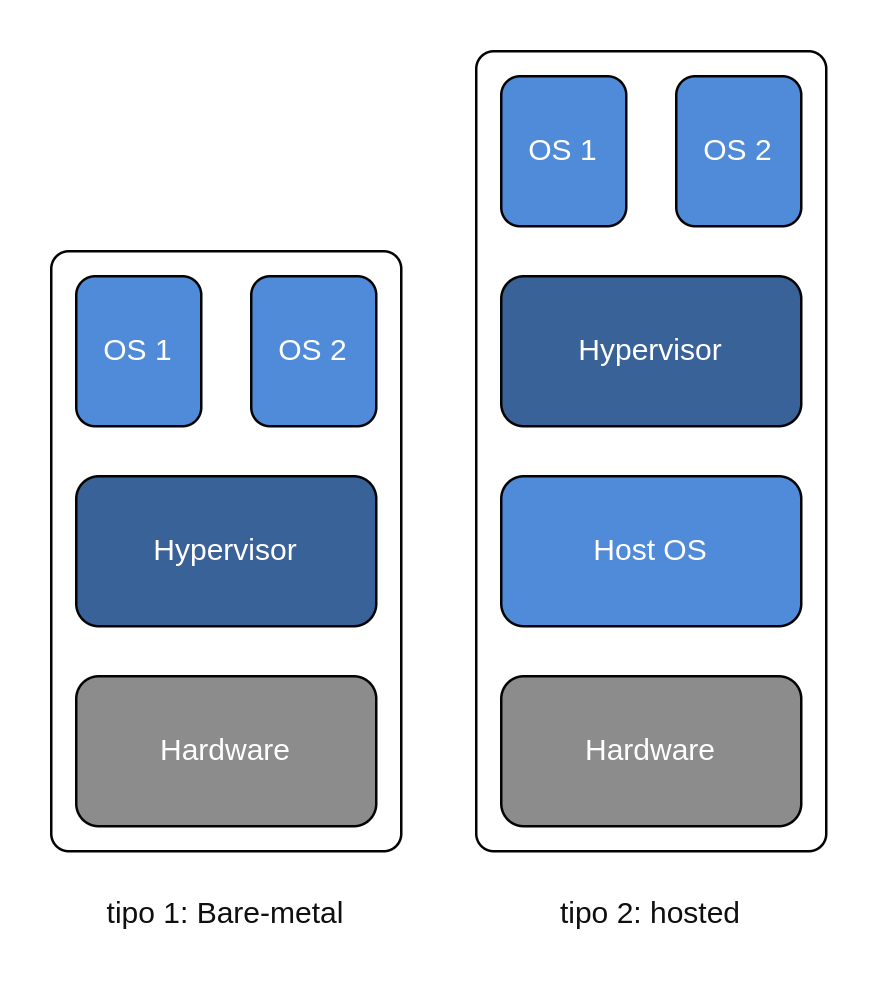
\includegraphics[width=8cm]{images/vm_t1_vs_t2.drawio.png}
    \caption{Virtualização tipo 1 vs tipo 2}
    \label{fig:virtualization_t1_vs_t2}
\end{figure}

\paragraph*{Tipo 1 - Bare-metal}\mbox{}\\
No tipo de virtualização bare-metal, temos o hypervisor que cuida de todo o gerenciamento do recurso e distribuição dos mesmos para cada SO convidado. Possuem performance melhor em comparação ao tipo 2, uma vez que seu acesso intercede exclusivamente o hypervisor, assim rodando praticamente de forma nativa, devido as camadas demonstrada na figura \ref{fig:virtualization_t1_vs_t2}.

A respeito deste tipo, o GNU/Linux implementa um módulo kernel-based virtualization machine (KVM), o qual resulta na capacidade de virtualização sobre este funcionar tal como um hypervisor. Deste modo, praticamente qualquer kernel Linux com este módulo pode ser utilizado tal como um hypervisor \cite{what-is-KVM}.

\paragraph*{Tipo 2 - Hosted Hypervisor}\mbox{}\\
Já no tipo 2, inicia-se um SO principal, e este através de virtualização de hardware e/ou tradução de interfaces binárias, possibilita o uso de recursos em um SO convidado. A comunicação do SO convidado com os recursos tende a ser mais demorada devido sua comunicação levar seu tempo de interpretação do SO principal, que por fim acessa o recurso solicitado, resultando assim em uma execução mais lenta quando comparado a virtualização tipo 1 bare-metal, conforme o aumento de camadas na figura \ref{fig:virtualization_t1_vs_t2}.


\section{Containers}
\label{chp:referencial_teorico::sct:containers}
Já na conteinerização, o processo é mais simples por disponibilidade de alguns recursos providos pelo GNU/Linux, os quais são os Namespaces e cgroups, que possibilitam gerenciar acesso e uso de recursos sem utilização de muitas abstrações utilizadas em uma MV (criação de um driver virtual). Além de todos os processos rodarem no mesmo SO, o qual pode ser verificado na máquina host como só mais um processo na árvore de processos, diferentemente de uma MV que aponta a existência de um único processo. Mais a respeito pode ser visto no tópico.

Os containers, basicamente utilizam recursos supracitados, para fazer o isolamento daquilo que seria disponível para o processo, em geral tratando-se de uma camada a qual não tem acesso irrestrito a recursos do SO, tais como pontos de montagem de arquivos, comunicação entre processos e entre outras funcionalidades \cite{what-container, what-are-container}.

Entretanto vale ressaltar que o processo roda isolado na percepção de si próprio, mas não da SO host do container, do qual tem livre acesso a tudo do processo dentro do container. Isto deve-se a questão deste estar rodando sob o SO host de forma nativa, diferentemente do que ocorre em MVs, resultando assim em inicialização do container de forma imediata.

Como visualização das diferenças entre os tipos de virtualização desde MVs a containers, temos a figura \ref{fig:container_vs_virt_t1_vs_virt_t2}.

\begin{figure}
    \centering
    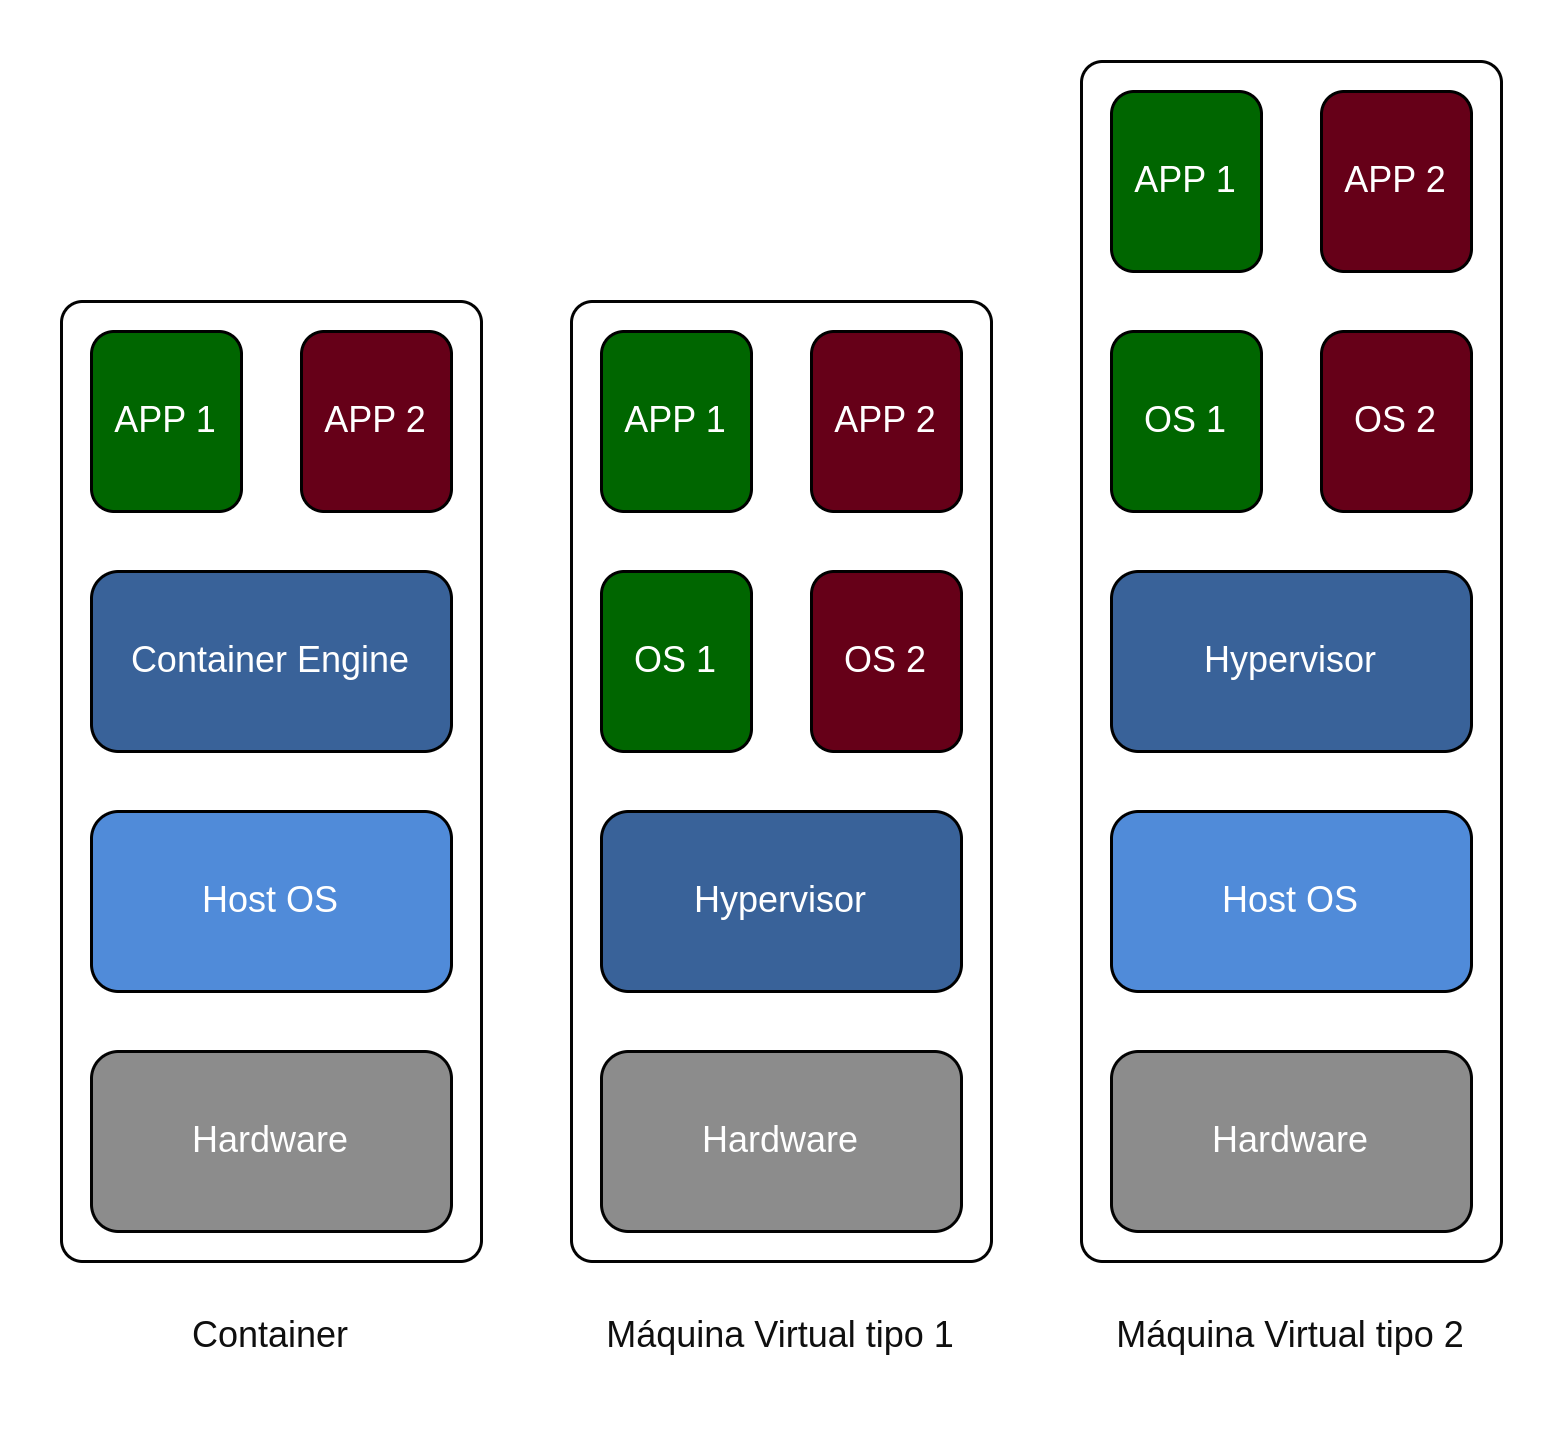
\includegraphics[width=11cm]{images/virt_container_vs_t1_vs_t2.drawio.png}
    \caption{Container vs Virtualização tipo 1 vs tipo 2}
    \label{fig:container_vs_virt_t1_vs_virt_t2}
\end{figure}

\section{Comparativo entre máquina virtual e container}
Em questão de comparação entre estes tipos de virtualização, MV e container, como visto, estas tem características inerentes neles que provém algumas qualidades e defeitos que vão ser cruciais para entendimento de qual caso de uso é mais adequado. Desta forma, como já fora previamente discorridos os conceitos, temos a seguinte tabela comparativa como demonstrativo direto de pontos fortes e fracos de cada solução.

\begin{tabular}{|c|p{5cm}|p{5cm}|}
\hline
\textbf{Parametro} & \textbf{Máquina Virtual} & \textbf{Container} \\
\hline
OS convidado    & Roda sobre hardware virtual e kernel é carregado em sua própria região de memória & Todos os convidados compartilham o mesmo kernel, e a imagem do kernel é carregado na memória física \\
\hline
Comunicação     & Será feita através de dispositivos de rede & Mecanismos padrões de IPC, como sinais, pipes, sockets, etc \\
\hline
Segurança       & Depende da implementação do Hypervisor & Mecanismos de controle do kernel \\
\hline
Performance     & Sofre do overhead das instruções a serem traduzidas do convidado para o host & Provém uma performance quase nativa \\
\hline
Isolamento      & Bibliotecas compartilhadas, arquivos e etc, não podem ser compartilhados entre convidado e host & Subdiretórios podem ser montados e compartilhados entre host e container \\
\hline
Tempo de inicio & Precisam de alguns minutos para iniciar  &  Podem ser iniciados em segundos \\
\hline
Armazenamento  & Precisa de muito armazenamento para seu kernel, programas e dependências &  Ocupam menos espaço uma vez que o kernel é compartilhado \\
\hline
\end{tabular}


